\subsection{CAN-card}	%Jonatan & Hampus
\noindent Two versions of the CAN-card is used, the one developed last year and a modified version of that one to be able to use six PWM signals on the same card. 

\begin{figure}[!ht]
	\begin{center}
		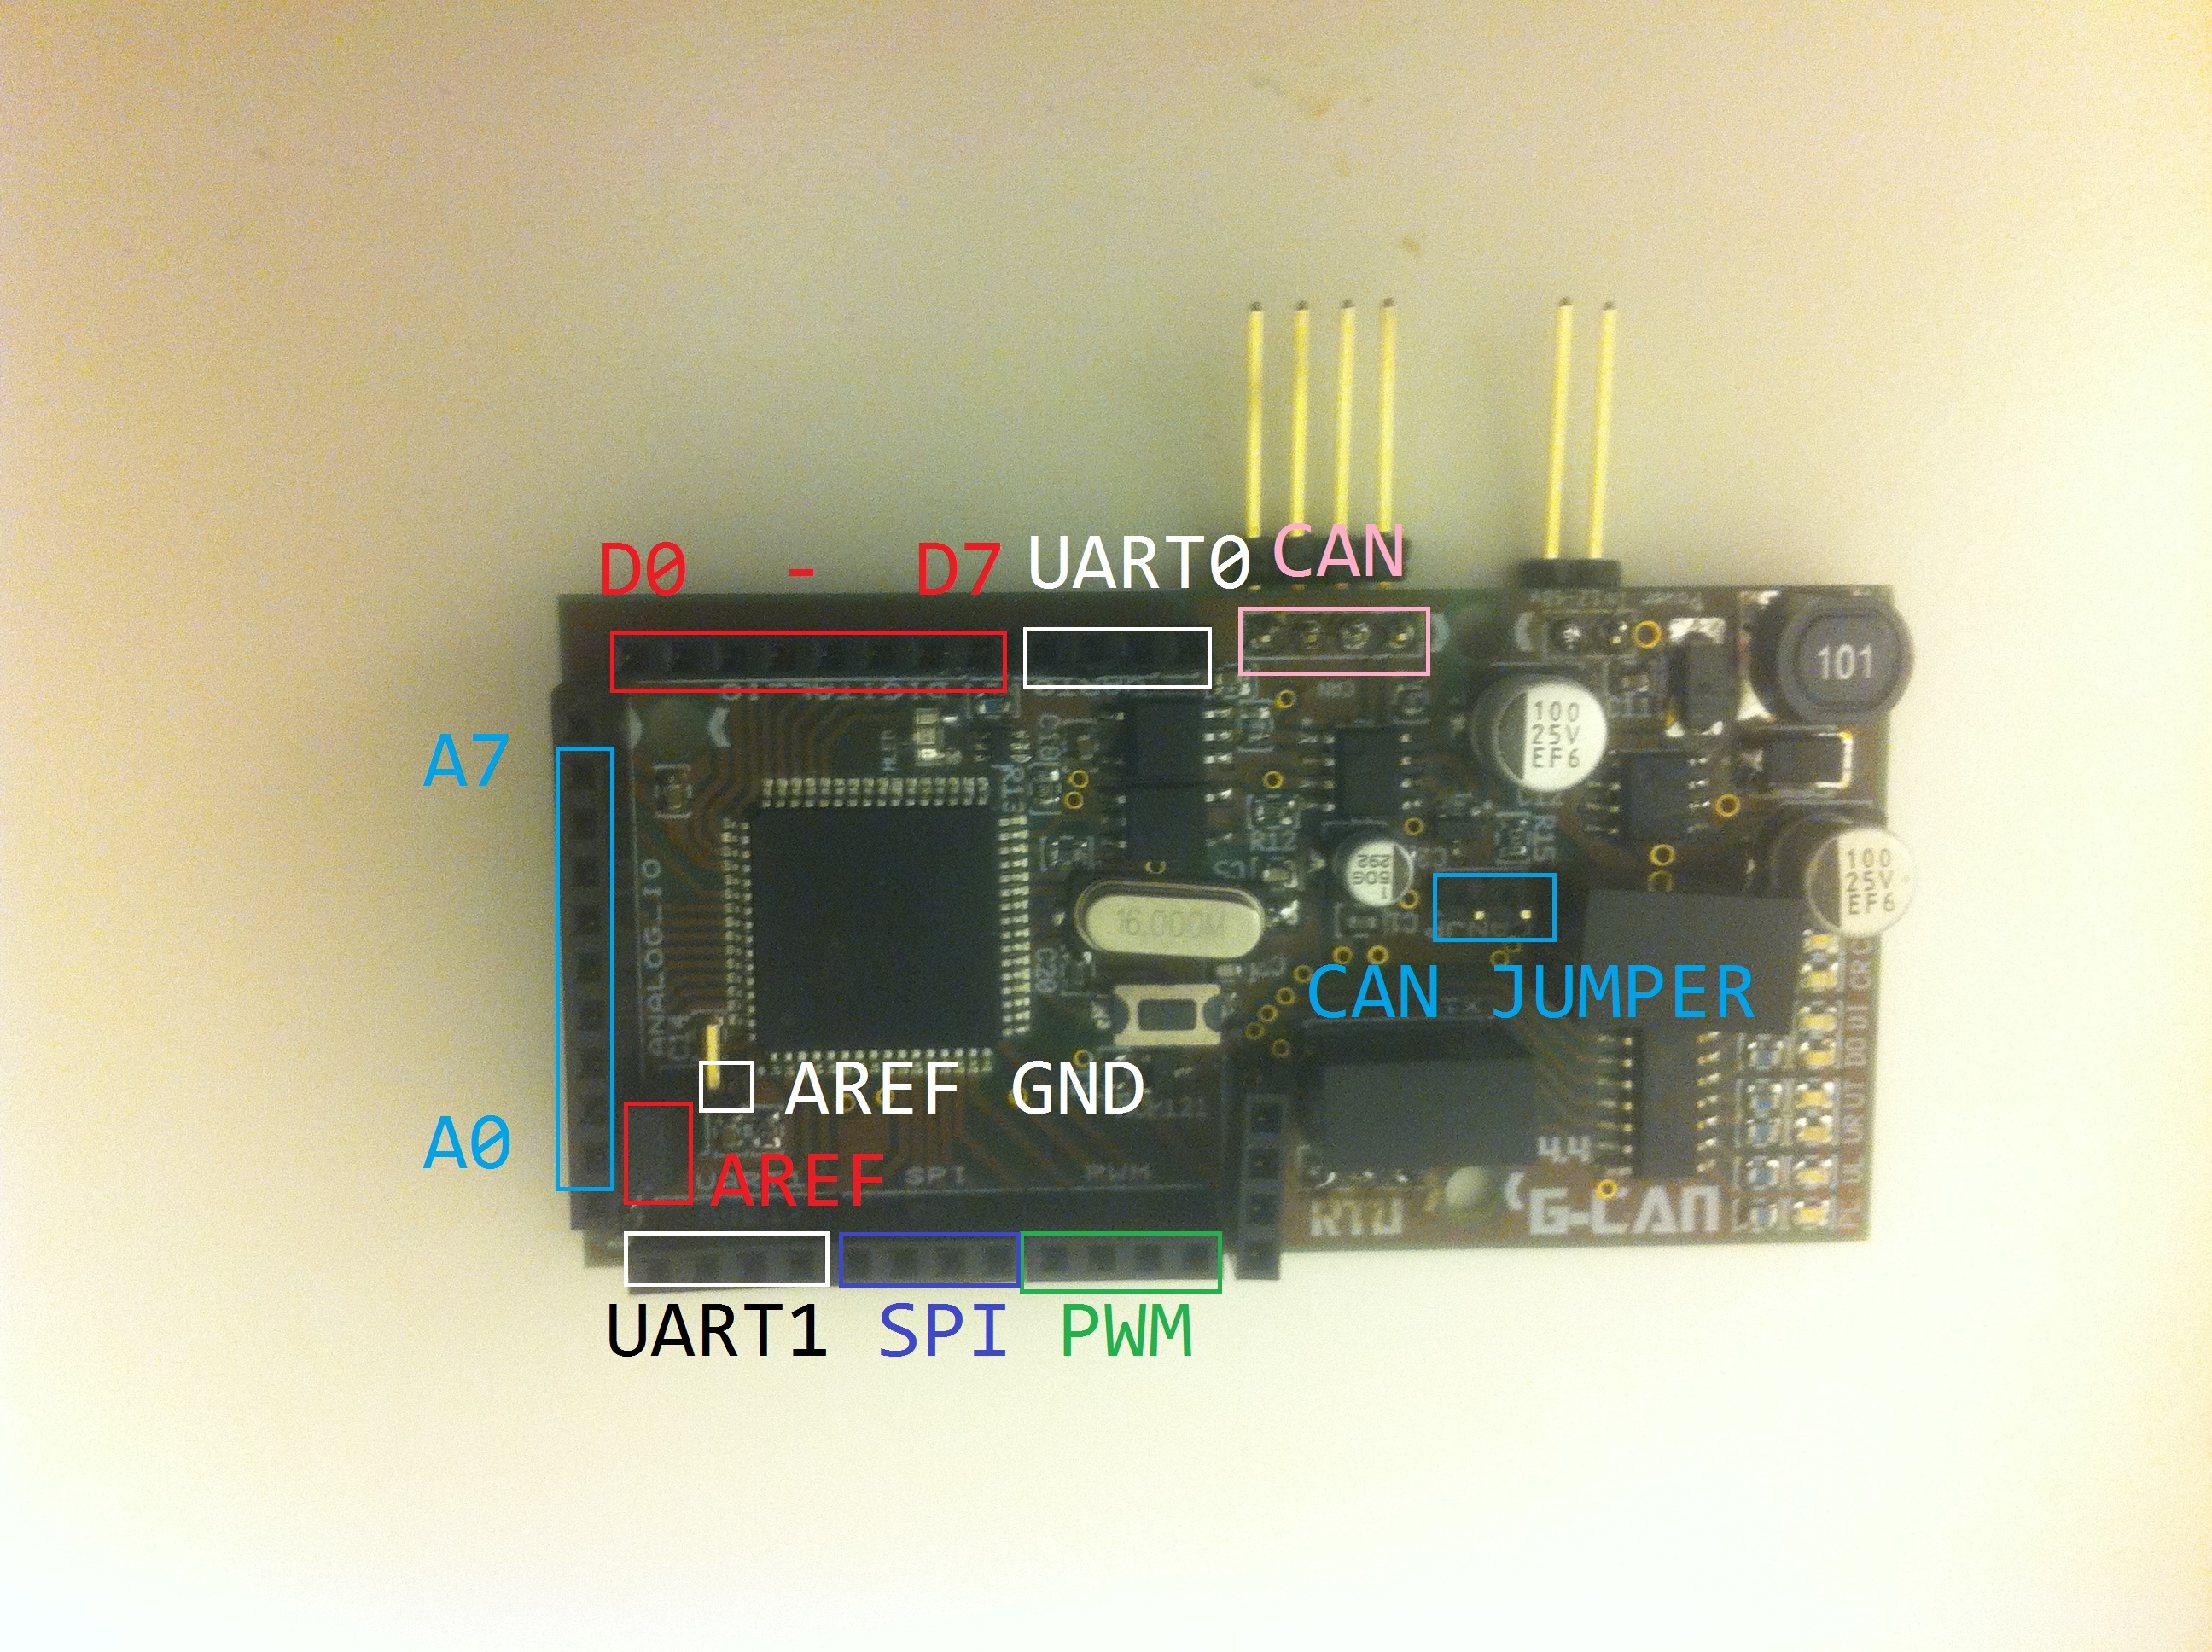
\includegraphics[width=80mm]{./Images/Software/gcan_v4_4.JPG}
		\caption{Generic CAN card version 4.4}
		\label{YourLabel}
	\end{center}
\end{figure}

\begin{figure}[!ht]
	\begin{center}
		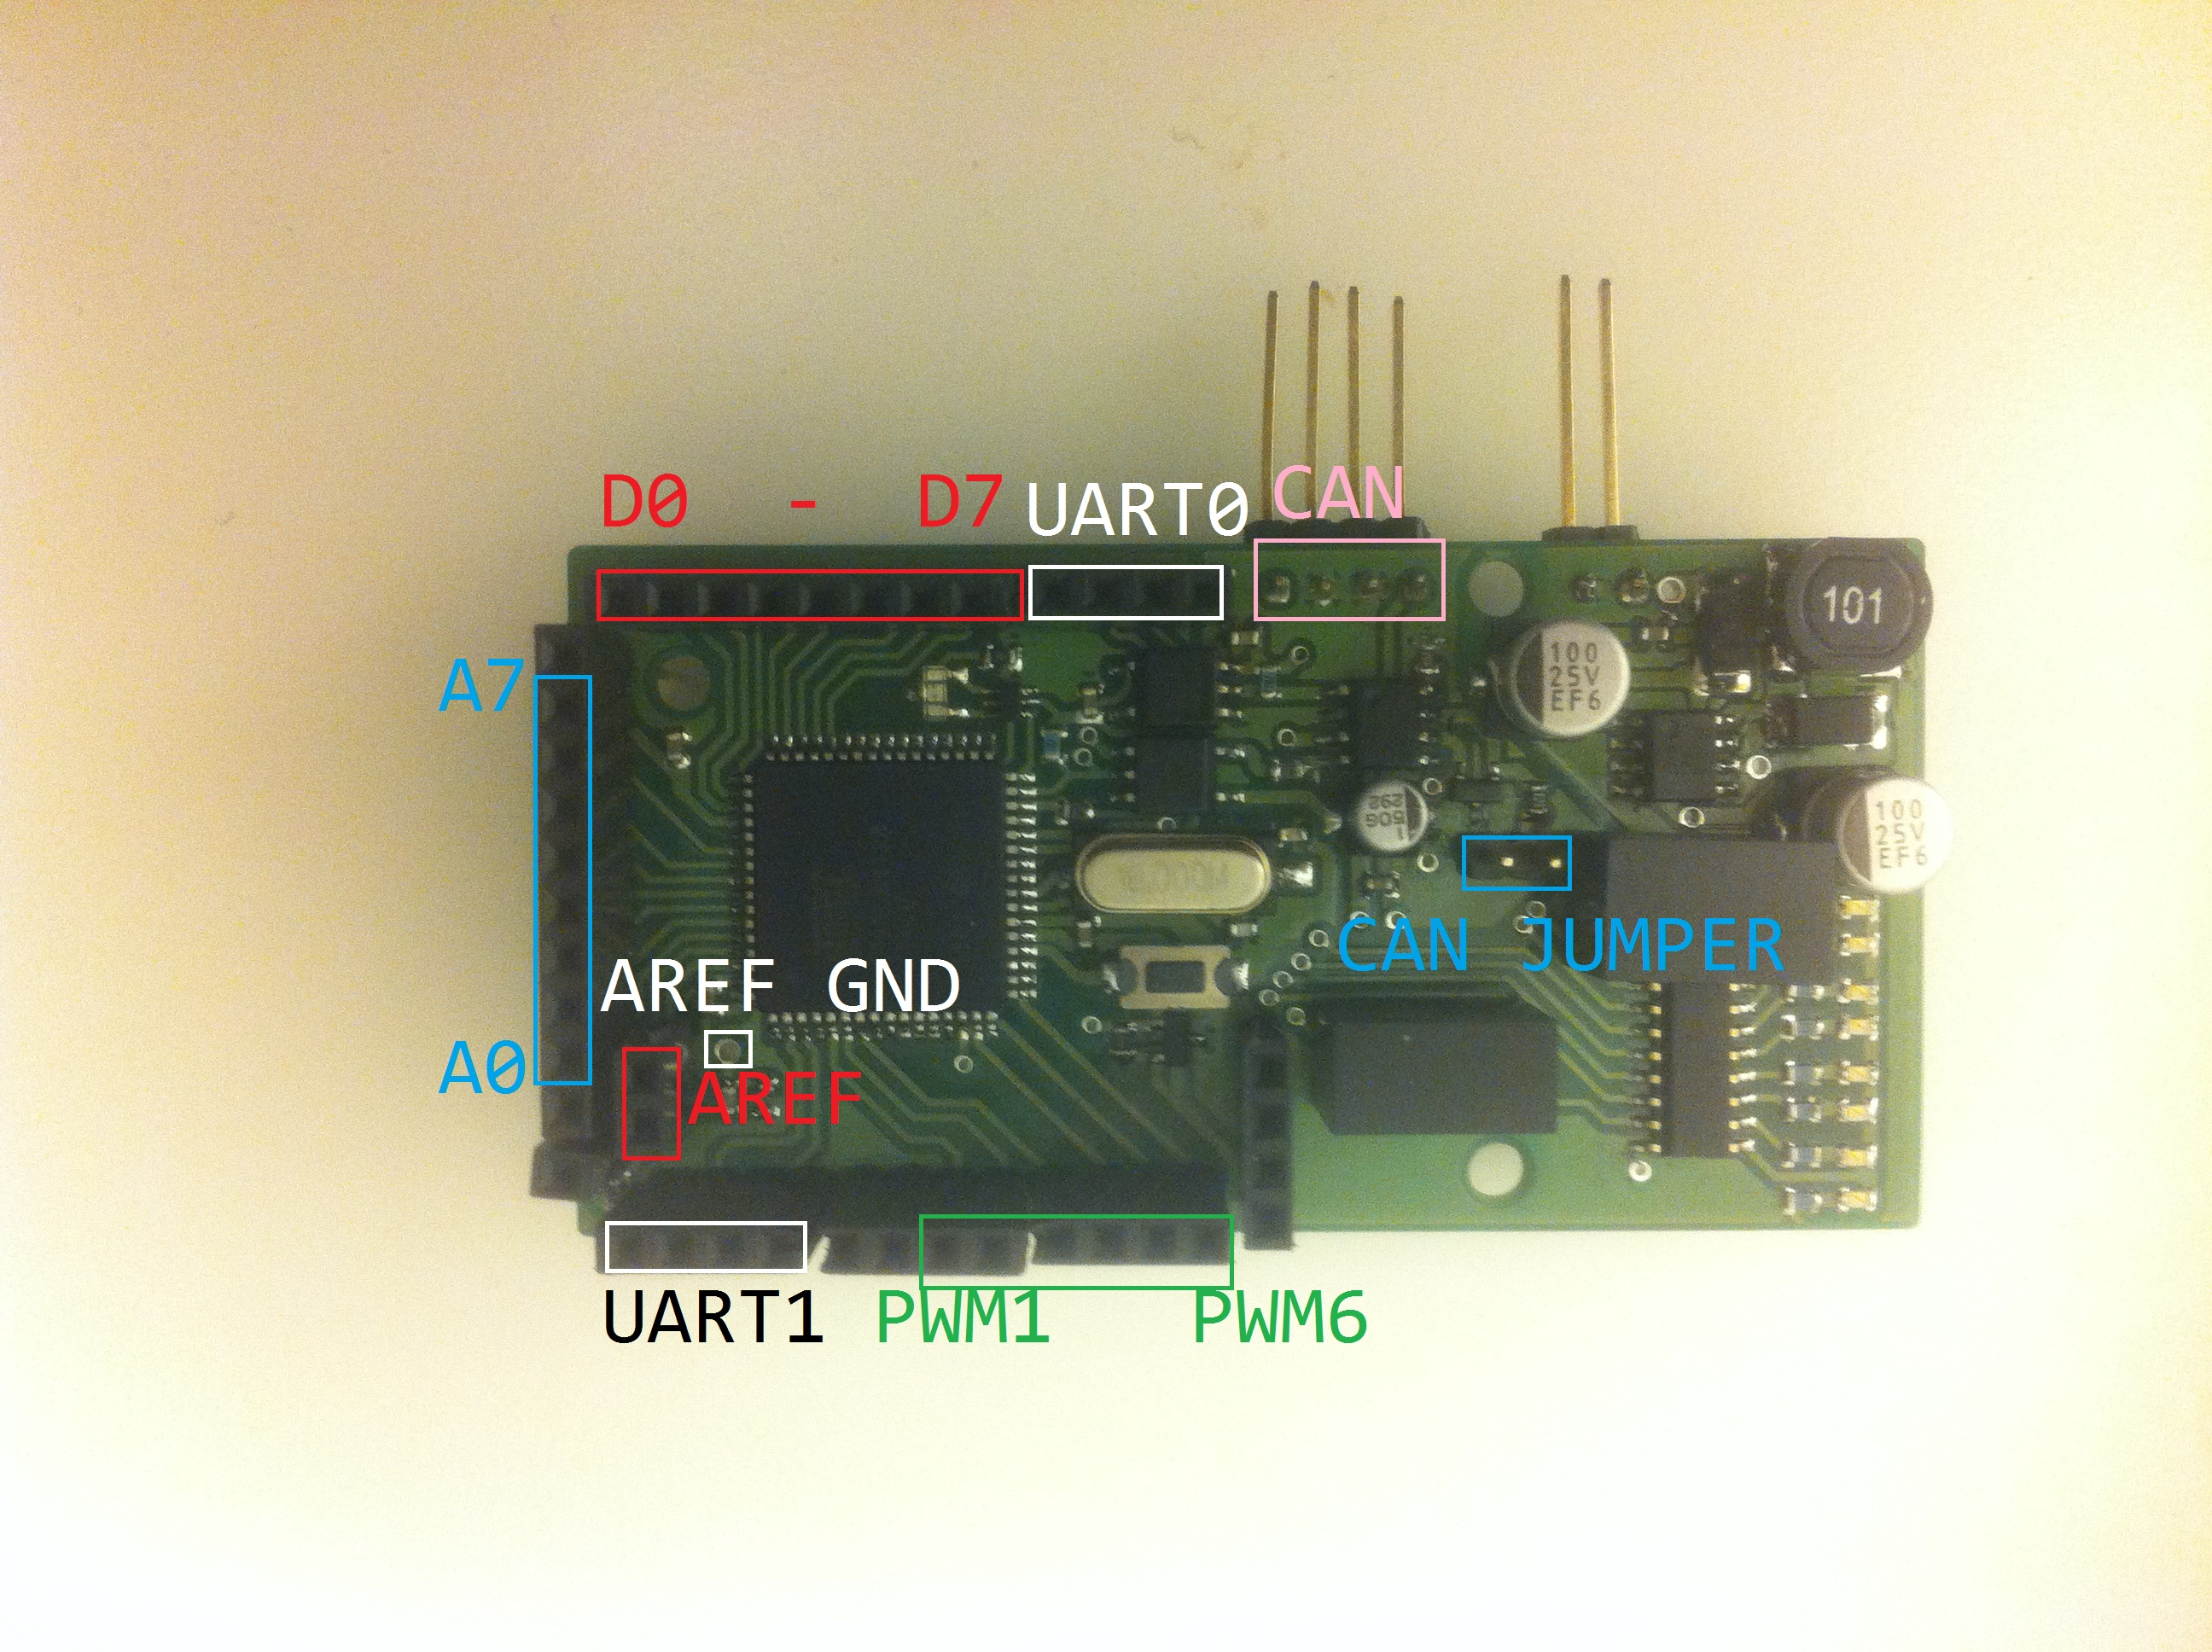
\includegraphics[width=80mm]{./Images/Software/gcan_v5_0.JPG}
		\caption{Generic CAN card version 5.0}
		\label{YourLabel}
	\end{center}
\end{figure}

To use the analog ports as analog inputs a jumper on AREF is required. For the CAN-bus to work it needs atleast one jumper over CAN Jumper pins in the pictures above, but more is not a problem, so preferably use one jumper on each card.
%label till bilder

The CAN-cards got Atmels microprocessor AT90CAN128 \cite{at90can128} coupled with a 16MHz oscillator. It got hardware support for Serial Peripheral Interface (SPI), Controller Area Network (CAN) and Universal asynchronous receiver/transmitter (UART) protocols. The AT90CAN128 microprocessor is programmed with the JTAGICE MKII\cite{JTAGICEMKII} or JTAGICE 3\cite{JTAGICE3} from Atmel or equivalent together with the software Atmel studio 6.
To program, attach the programmer to the analog pins. 
\subsubsection{Thruster node}
\noindent From the previous years requirement one micro controller should be assigned to each motor. This requirement was removed this year which lead to the decision to let all motors become one node with a mutual micro controller, saving both energy, reducing heat and lessen the load on the CAN-bus.
The PWM signal for the motors runs on 50 Hz and a duty cycle between 5\% and 15\%. The cards receives instructions from CAN messages where a byte of data represents the desired speed.

\subsubsection{Sensor node}
\noindent The sensor node handles all the analog sensors such as the pressure sensor \cite{Pressure_sensor}, the temperature sensor and the salinity sensors. For the time being, only the pressure sensor has been implemented. It is able to give the depth of the unit down to three bars pressure which translates to roughly 20 meters.
A temperature and at least one salinity sensor is planned to be implemented as well in the future to help the system estimate movement etc.
First an sample from the pressure sensor should be taken to measure the value at the surface, the analog-digital-converter (ADC) has a resolution of 10 bits, therefore the resolution of the depth would be 
\begin{equation}\label{first}
20 metres / 2^{10} = 20 000 centimetres / 1024 = cm depth / analog value \approx 2 cm / 1 analog value
\end{equation}


So the real depth of Naiad would be 
\begin{equation}\label{first}
(current value - initial value) * 2 = centimetres below surface
\end{equation}
\subsubsection{Inertial navigation system node}

% Hampus
\noindent The main purpose of the INS card is to get the current orientation of Naiad. This is done thanks to an IMU and a fiber optic gyroscope. The IMU is communicating with UART. The IMU can be configurated to give a variance of data. Currently the outputting orientation in X, Y and Z axis as well as the true body acceleration in X, Y and Z. The output data of the IMU is sent as a string of characters containing both header information and the data itself. The INS card removes all of the header information by extracting specific sections of the string and converting them to float values. This heavily reduces the data that has to be transmitted and it makes the values possible to use immediately. As each float is four bytes and a CAN message can has eight bytes of data, each message can hold two values from the IMU. A total of three messages are required to send all the data for each time the IMU generates an output. The current IMU output frequency is 20Hz. An issue with the IMU is that it can drift in yaw due to the nature of the implementation of the IMU hardware. 

To compensate, a fiber optic gyroscope is added to track the yaw orientation. The fiber optic gyroscope is generating an output voltage correlated to the angular velocity around yaw. This voltage has to be measured very precisely which is why it is connected to an external low noise ADC. The ADC is sending the voltage value via SPI, this allows for a high bit rate which is needed to get a small integration interval. The ADC is acting as a slave in the SPI communication and it requires to first be selected through a slave select pin by pulling the voltage to a digital low. When the ADC is activated, it requires an external clock to drive the transmission. The clock should be starting with a rising edge when transmitting data. The initial procedure of the CAN-card is to send instruction to set the sample frequency of the ADC and also tell it to send data continuously so the CAN-card can avoid asking for data each time. As the ADC uses 24 bits to store the voltage value, each measurement has to be sent over three transmissions as the word size of the SPI is eight bits. The CAN-card will turn the slave off by turning the slave select pin to a digital high. 

\subsubsection{Power supply unit node}
\noindent This node controls how and when to start electronics and motors and also feedback to and from outside the robot in form of an LCD screen and a remote control. By controlling power to other nodes it has the possibility to restart the whole system on command or if needed.
The mission switch is connected to this node, by removing the switch it will send a command to the BBB allowing them to run the mission, if put back during a mission, the mission is paused until the switch is removed.
\subsubsection{Translator node}
\noindent Naiad mainly uses two different communication protocols to communicate between nodes, CAN and TCP. The link between them is UART as the BBB do not support the high voltage of the CAN-bus. The only task for this card is to read all the messages on the CAN-bus and pass them on to a BBB via UART and, vice versa, it translates UART messages to CAN messages. If this card sends too many UART messages over a short amount of time to a BBB, the BBB can crash.  
\subsubsection{LED node}
\noindent When the robot is in the water, debugging and understanding the system by reading the LCD is hard, so by being able to control a total of 4 rows, 2 on each wing, of RGB LEDs, a better understanding is achieved and it will draw more attention to the robot.
The card is also controlling power of the headlights in the front and bottom to support the vision system.
\subsubsection{Hydrophone node}
\noindent As the time difference between the signal generated from the different hydrophones is small, the time stamping for each is based on four different interrupts to avoid busy waiting. When all four interrupts are triggered, a calculation can be made to get the source direction of the sound. The direction calculation is not implemented. When an interrupt is triggered, the interrupt on that pin is disabled. This is required because the CAN-card will get multiple pulses from the same source instance. The interrupt pin is enabled when either all four interrupts have been triggered or after a set time.

%\subsubsection{Speed logger node}
%\noindent 
